%
% Unless otherwise indicated, the copyright in this material is 
% owned by Joerg Evermann. This material is licensed to you under the 
% Creative Commons by-attribution non-commercial license (CC BY-NC 4.0)}
%
\section*{Learning Goals}

After reading this chapter, you should be able to:
\begin{itemize}
   \item Create and manipulate basic data structures in R, including arrays, matrices, and data frames.
   \item Create summary information from R data frames and other data structures.
   \item Use the Tidyverse packages to retrieve information from R data frames, including filtering, grouping, and aggregation of information.
   \item Use SQL to operate on R data frames to retrieve information, including filtering, grouping, and aggregation of information.
\end{itemize}

\section{Introduction}

R is a highly acclaimed statistical software and programming language known for its robust capabilities in data analysis, visualization, and statistical computing. It was conceived in the early 1990s by Ross Ihaka and Robert Gentleman at the University of Auckland, New Zealand. Drawing inspiration from the S language developed at Bell Laboratories, R was designed to be a powerful and flexible tool for data analysis and statistical modeling.

One of the key advantages of R is its open-source nature, making it freely available to users worldwide. This accessibility has fostered a vibrant community of users and developers, continuously enhancing its functionality through comprehensive packages and extensions. The Comprehensive R Archive Network (CRAN), a repository of these packages, is a testament to R's extensible architecture, offering tools for a myriad of data analysis tasks.

R's popularity stems not only from its wide range of statistical techniques, including linear and nonlinear modeling, time-series analysis, classification, clustering, and others, but also from its exceptional capabilities in data visualization. The software provides an integrated suite of tools for data manipulation, calculation, and graphical display, making it an invaluable asset for statisticians, researchers, and data scientists.

Moreover, R's programming language aspect allows for automation and customization in data analysis, which is highly beneficial for complex and repetitive tasks. Its compatibility with various data formats and integration with other programming languages and tools further enhances its versatility.

\section{Using R}

R is a command-line oriented software, that is, users type commands to perform calculations or call functions of R packages. A sequence of R commands can be assembled in a \emph{script file}, so that they may be re-run when necessary. The advantage of this type of software over one with a graphical user interface is in the repeatability and replicability of the work. Ideally, data analysts will assemble an R script file for their entire data analysis, from raw data sets to finished statistical analyses and visualizations, so that all details of the analysis are available for replication and evaluation.

\begin{figure}
\centering
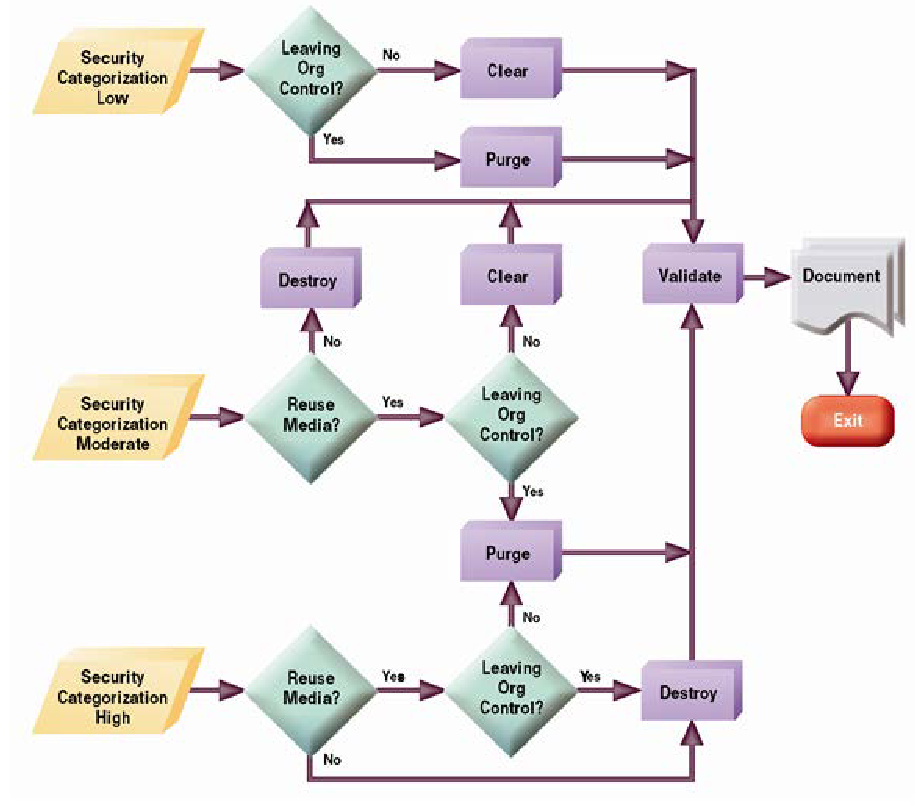
\includegraphics[width=.8\textwidth]{screen1.png}
\caption{The R command line interface}
\label{fig:r}
\end{figure}

The R system can be launched simply by invoking the \texttt{R} command from the terminal window, as shown in Figure~\ref{fig:r}. R will display its version information and prompt for command entry with a \texttt{>} prompt. 

To install R on Microsoft Windows or on MacOS, download the installation files from CRAN (Comprehensive R Archive Network) at \url{https://cran.r-project.org} and follow the instructions. R on Microsoft Windows and R on MacOS will show their command prompts inside a window but otherwise function similarly to R on Ubuntu that is installed in the course virtual machine.

\begin{tcolorbox}[colback=alert]
\paragraph*{Tip:}
A good, easy, and comprehensive introduction to R can be found here: \url{https://cran.r-project.org/doc/manuals/r-release/R-intro.pdf}
\end{tcolorbox}

\begin{tcolorbox}[colback=code]
\paragraph*{Tips for working efficiently with R:}

To make using R more efficient, consider doing the following:

\begin{itemize}
    \item Use the \colorbox{lightgray}{up-arrow} key to retrieve earlier commands.
    \item The \texttt{history()} function shows your command history.
    \item Use a notepad app to assemble your commands, then copy/paste to R.
    \item Use a notepad app for your results, copy/paste from R.
    \item The Ubuntu terminal window uses \colorbox{lightgray}{SHIFT-CTRL-X}, \colorbox{lightgray}{SHIFT-CTRL-C}, \colorbox{lightgray}{SHIFT-CTRL-V} for cut/copy/paste.
    \item Use multiple terminal and R windows (e.g. one for executing commands, one for reading help documentation or for listing files).
    \item Don't update packages in the middle of a project.
    \item Ensure you have a \emph{repeatable, automatable script} for your entire data analysis at the end of a project.
\end{itemize}

\end{tcolorbox}


\section{R Basics}

The most basic way to use R is to simply use it as a calculator, as shown in the following R code example. Type ''\texttt{1+1}'' at the ''\texttt{>}'' prompt, then press the \colorbox{lightgray}{RETURN} key to execute the statement. R will respond on the following line with the result:

\begin{samepage}
\begin{Rcode}
> 1+1
[1] 2
\end{Rcode}
\end{samepage}

A \emph{variable} in R is a named storage space for numbers, characters, strings, and other data elements. Traditionally, values are assigned to variables using the \texttt{<-} operator, but one may also use the more ''normal'' assignment operator \texttt{=}. Using the \texttt{<-} assignment operator helps to clearly distinguish assignment from equality testing, which uses \texttt{==}. 

The following R code example introduces the R function called \texttt{print()} that does as its name suggests. Most data types and data structures that can be assigned to variables have a useful print function associated to them, so that on the interactive R command line you can simply type their name to get their value. In interactive mode, R calls the \texttt{print()} function automatically, in an R script that you execute from file, you will have to exiplictly use the \texttt{print} function.

\begin{samepage}
\begin{Rcode}
> a <- 3
> b <- 2
> print(a * b)
[1] 6
> a
[1] 3
\end{Rcode}
\end{samepage}

A common structured data type in R is a \emph{vector}\index{Vector (in R)}. A vector in R contains elements of the same data type and is ordered. When assigning elements of different datatypes to a vector, R will coerce the types of all elements to a common datatype.

\begin{samepage}
\begin{Rcode}
> v <- c(1, 'a', TRUE)
> v
[1] "1"    "a"    "TRUE"
> v <- c(1, 2, 3, 4)
> v*3
[1]  3  6  9 12
\end{Rcode}
\end{samepage}

Note that R automatically determined that multiplication with a scalar is an element-wise operation and applies it to each element of the vector. 

Useful functions to create vectors are the sequence function \texttt{seq()}, which accepts the lower and upper limit and a step size as parameter, and the repetion function \texttt{rep()} which repeats its first argument the number of times specified by its second argument.

\begin{samepage}
\begin{Rcode}
> s <- seq(0, 6, by=.5)
> print(s)
> r <- rep(3.5, 5)
> print(r)
\end{Rcode}
\end{samepage}

R provides useful functions for numerical vectors, to find their length, their maximum and minimum value, the square root of their values, as well as the variance and standard deviation of the elements. Note that R automatically determines whether functions are applied to the whole vector, like \texttt{var()} or \texttt{sd()}, or whether functions are applied element-wise to each element, like \texttt{sqrt()}. Vector concatenation, using the \texttt{c()} function, automatically ''flattens'' the vectors.

\begin{samepage}
\begin{Rcode}
> length(v)
> max(v)
> min(v)
> sqrt(vv)
> var(v)
> sd(v)
> vv <- c(v, c(7, 8, 9), v)
> print(vv)
\end{Rcode}
\end{samepage}

The most common way to select elements from vectors is by \emph{indexing} with a boolean vector. In the following example, the expression \texttt{vv < 5} yields a vector of boolean values. Indexing the variable \texttt{vv} with that vector determines which elements of \texttt{vv} to select.

\begin{samepage}
\begin{Rcode}
> vv < 5
> vv[vv < 5]
> vv[vv < 5] <- vv[vv < 5] + 5
\end{Rcode}
\end{samepage}

Vectors can also be indexed numerically, selecting elements by their position. R allows you to specify a sequence using the \texttt{:} operator and exclusion of elements using \texttt{-}, sometimes called slicing\index{Slicing}. The first line in the following example selects elements at positions 3 through 7, the second line selects elemtns \emph{except} those at positions 3 through 7.

\begin{samepage}
\begin{Rcode}
> vv[3:7]
> vv[-(3:7)]
\end{Rcode}
\end{samepage}

\begin{tcolorbox}[colback=alert]
\paragraph*{Important:}
\begin{itemize}
   \item R begins indexing positions with 1, while other programming languages begin at 0.
\end{itemize}
\end{tcolorbox}

\begin{tcolorbox}[colback=code]
\paragraph*{Tip:}
\begin{itemize}
   \item The boolean constants \texttt{TRUE} and \texttt{FALSE} can be abbreviated by \texttt{T} and \texttt{F}
\end{itemize}
\end{tcolorbox}

R also has special symbols to denote infinity (\texttt{inf}) and results that are not a number (\texttt{NaN}):

\begin{samepage}
\begin{Rcode}
> 2 / 0
[1] Inf
> 0 / 0
[1] NaN
\end{Rcode}
\end{samepage}

Importantly, \texttt{NaN} is \emph{not} the same as a missing value, which is denoted by \texttt{NA}, as in the following R code example. The \texttt{is.na()} function can be used to identify and index \texttt{NA} and then filter them. Any \texttt{NA} typically yields an \texttt{NA} when an aggregate function is applied. Many functions offer an option to remove \texttt{NA} values prior to applying them, as shown for the \texttt{sum()} function in the following R code block. 

\begin{samepage}
\begin{Rcode}
> v[3] <- NA
> v*3
[1]  3  6 NA 12
> is.na(v)
[1] FALSE FALSE  TRUE FALSE
> sum(v)
[1] NA
> sum(v, na.rm=TRUE)
[1] 7
\end{Rcode}
\end{samepage}

\noindent The boolean logical \emph{and} and \emph{or} are represented by the operators \texttt{\&} and \texttt{|} shown in the R code block below.

\begin{samepage}
\begin{Rcode}
> TRUE & FALSE
FALSE
> TRUE | FALSE
TRUE
\end{Rcode}
\end{samepage}

Character strings in R are enclosed in single or double quotes (but not mixed quotes!). Two useful functions are \texttt{paste()} which pastes its arguments together with an optional separator between them and returns a characters string, and the \texttt{strsplit()} function which accepts a string (or vector of strings) to split, and a separator character that identifies where to split the string. It returns a list of vectors of strings.

\begin{samepage}
\begin{Rcode}
> label1 = 'I Love R'
> label2 = 'and BUSI 4760'
> paste(label1, label2, sep=' ')
> strsplit('Hello World! My first string', ' ')
\end{Rcode}
\end{samepage}

Because you can assign arbitrary values to variables in R, R provides functions to test the value type and to change or coerce the value type. A \emph{factor}\index{Factor (in R)} data type in R represents categorical data, encoded as different character strings or different numbers. Categorical data is treated different from numerical or character string data in many statistical analyses.

\begin{samepage}
\begin{Rcode}
> is.numeric(vv)
> is.integer(vv)
> mode(vv)
> as.character(vv)
> is.character(as.character(vv))
> as.factor(as.character(vv))
> levels(as.factor(as.character(vv)))
\end{Rcode}
\end{samepage}

Important string functions are \texttt{grep()}, which checks whether strings contain a substring that matches a regular expression, and \texttt{agrep()}, which calculates the Levenshtein distance between a regular expression and a set of strings. The Levenshtein distance is defined as the sum of insertions, deletions, and substitutions of characters to transform one string into another. The first use of \texttt{grep()} in the following R code block matches a phone number, the second use of \texttt{grep()} matches a Canadian postal code, while the last two examples of \texttt{grep()} and \texttt{agrep()} exemplify the difference between exact matching with \texttt{grep()} and approximate matching with \texttt{agrep()}.

\begin{samepage}
\begin{Rcode}
> grep('^([0-9]{3})[ -]?[0-9]{3}[ -]?[0-9]{4}$', 
    c('709 864 5000', 'abc def 9999', '709-865-5000'))
[1] 1 3
> grep('[A-V][0-9][A-V] [0-9][A-V][0-9]', 
    c('A0P 1L0', '0AB L2K', 'A0X 1Z0'))
[1] 1
> grep('apple', c('apricot', 'banana', 'grape', 'pineapple'))
[1] 4
> agrep('apple', 
    c('apricot', 'banana', 'grape', 'pineapple'), 
    max.distance=3)
[1] 1 3 4
\end{Rcode}
\end{samepage}

\section{The R Environment}

The collection of variables, functions and libraries that exists in R at any one time is called the R \emph{workspace}. R provides many functions to manipulate objects in its workspace, among them \texttt{ls()} and \texttt{rm()}, named after their Unix bash shell equivalents. The following R code illustrates the use of these functions. Results may vary depending on what variables have been created prior to these commands.

\begin{samepage}
\begin{Rcode}
> ls()
[1] "a"          "b"          "v"
> rm(v)
> ls()
[1] "a"          "b"
\end{Rcode}
\end{samepage}

R comes with a built-in user manual that one can access with the \texttt{help()} function or simply the \texttt{?} operator. Help is available on any function in R, as shown in the following example. For added convenience, R provides a web browser interface to its help pages that is started by \texttt{help.start()}.

\begin{samepage}
\begin{Rcode}
> help()
> help(lm)
> ?lm
> ??lm
> help.start()
\end{Rcode}
\end{samepage}

R has a working directory where it reads and writes files from and to. On Ubuntu Linux, this is the directory from which the \texttt{r} command was issued. R provides functions to get the working directory, to set (change) it, and to list the files in the working directory:

\begin{samepage}
\begin{Rcode}
> getwd()
[1] "/home/busi4720"
> setwd('DataSets')
> getwd()
[1] "/home/busi4720/DataSets"
> list.files()
\end{Rcode}
\end{samepage}

\begin{tcolorbox}[colback=code]
\paragraph*{Tip:} It is often more convenient to change the working directory in the terminal, prior to invoking \texttt{r}.
\end{tcolorbox}

A collection of related functions is called a \emph{library} in R. While some libraries come with the base R system, other packages will need to be downloaded and installed. The CRAN (comrehensive R archive network) provides libraries in convenient form. To install packages from CRAN, use the \texttt{install.packages()} which accepts the name (or a vector of names) of packages to install from CRAN. On some systems, R may prompt the user from which CRAN location to install packages. Normally, there is little difference other than download speed. 

Installed libraries can be attached to the R workspace with the \texttt{library()} function. The \texttt{library()} function with an argument attaches the specified package and makes its functions and data sets available for use. The \texttt{library()} function without any arguments shows which libraries are installed. The \texttt{search()} function shows which packages are currently attached to the workspace. Finally, \texttt{installed.packages()} provides details of all installed packages. 

\begin{samepage}
\begin{Rcode}
> search()
> library(matrixcalc)
> search()
> library()
> install.packages('lavaan')
> library()
> installed.packages()
\end{Rcode}
\end{samepage}

It is sometimes useful to assemble a set of related R commands in a script file. As noted earlier, script files are useful to improve the replicability of the data analysis. The \texttt{source()} function will read and execute a file containing R commands. As noted earlier, in a script file, you will need to use the \texttt{print()} function to print the values of variables.

\begin{Rcode}
> source('MyFirstScript.R')
\end{Rcode}

Finally, the \texttt{quit()} function ends an R session. When using \texttt{quit()} without arguments, R will ask whether to save the workspace image. R stores its \emph{workspace} in each directory in a file called ''.RData'' and will read it when restarted from that directory. R also stores its \emph{command history} in each directory in a file called ''.Rhsitory'' and will read it when restarted from that directory.

\begin{Rcode}
> quit()
\end{Rcode}

\section{Arrays, Matrices, Lists, and DataFrames}

R \emph{arrays}\index{Array (in R)} are multi-dimensional objects that can hold any primitive data type, usually numerical. A \emph{matrix}\index{Matrix (in R)} is simply a two-dimensional array. The following example shows how indexing generalizes from vectors to matrices and arrays simply by indexing each dimension with the same syntax as used for vectors. The \texttt{array()} creates multi-dimensional arrays from existing data, the \texttt{dim()} function returns the number of dimensions of an array.

A few important things to note in the following R code block example:
\begin{itemize}
   \item Initially, the array is created from a range of numbers between 1 and 20, and the \texttt{dim} argument specifies the dimensionality. 
   \item A dimension need not be subsetted or indexed, as in \texttt{a[,2]} or \texttt{a[,2:4]} which do not subset the first dimension
   \item Reversing the index reverses the result that is returned, as in \texttt{a[3:1,2:4]} which reverses the indexing of the first dimension. 
   \item An array with two columns is interpreted as a set of indexes, as in \texttt{a[i] <- 0}
\end{itemize}

\begin{samepage}
\begin{Rcode}
> a <- array(1:20, dim=c(4,5))
> a
     [,1] [,2] [,3] [,4] [,5]
[1,]    1    5    9   13   17
[2,]    2    6   10   14   18
[3,]    3    7   11   15   19
[4,]    4    8   12   16   20
> dim(a)
[1] 4 5
> a[,2]
> a[,2:4]
> a[3,2:4]
> a[3:1,2:4]
> i <- array(c(1:3,3:1), dim=c(3,2))
> a[i] <- 0
> a
\end{Rcode}
\end{samepage}

Constructing a \emph{matrix} with the \texttt{matrix()} function is similar to constructing an array, but instead of providing the dimensionality with \texttt{dim}, one must provide the number of rows or colums (\texttt{nrow} or \texttt{ncol}) and how to fill the matrix from the elements provided using the \texttt{byrow} argument. The \texttt{t} function returns the transpose of a matrix, that is, it reverses rows and columns. Binding two matrices together by columns with \texttt{cbind()} or by rows with \texttt{rbind()} requires compatible dimensions.

\begin{samepage}
\begin{Rcode}
> b <- matrix(20:1, nrow=5, byrow=T)
> b
     [,1] [,2] [,3] [,4]
[1,]   20   19   18   17
[2,]   16   15   14   13
[3,]   12   11   10    9
[4,]    8    7    6    5
[5,]    4    3    2    1
> is.matrix(b)
> is.matrix(a)
> t(b)
> cbind(a, t(b))
> rbind(t(a), b)
\end{Rcode}
\end{samepage}

A \emph{list}\index{List} in R is an ordered collection of elements that, in contrast to vectors, \emph{may be of different types}. Lists are created using the \texttt{list()} function. Note the difference in selecting elements: The \texttt{[[]]} operator returns the element at that position in the list, whereas the \texttt{[]} operator contains a list that contains the element at that position in the list. 

\begin{samepage}
\begin{Rcode}
> l <- list('a', 3, 'b', 2, TRUE)
> l[[2]]
> l[2]
> is.list(l)
> is.list(l[[2]])
> is.list(l[2])
> as.list(vv)
\end{Rcode}
\end{samepage}

A \emph{data frames}\index{Data frame!in R} are the most widely used data structure for data analytics and statistics in basic R. It is essentially a table with a set of columns whose elements are of the same type. Columns are named and columns can be selected using the \texttt{\$} symbol. Useful functions on data frames are \texttt{summary()}, \texttt{head()} and \texttt{tail()}. The following R code block creates a variable \texttt{x} as a vector of 50 normally distributed random values using the \texttt{rnorm()} function. The variable \texttt{y} is created from vector \texttt{x} and additional normally distributed random variables. The two are then combined into a data frame. The \texttt{colnames()} function can retrieve the column names, but can also be used to change/update the column names. The \texttt{nrow()} and \texttt{ncol()} functions return the number of rows and columns, \texttt{head()} and \texttt{tail()} return the first few or last few rows, and \texttt{cov()} is an example of a statistical function that returns the covariance matrix of all columns in the data frame.

\begin{samepage}
\begin{Rcode}
> x <- rnorm(50)
> y <- 2*x + rnorm(50)
> data <- data.frame(x, y)
> colnames(data)
> colnames(data) <- c('Pred', 'Crit')
> nrow(data)
> ncol(data)
> data$Pred
> summary(data)
> head(data)
> tail(data)
> cov(data)
\end{Rcode}
\end{samepage}

Data frames may be written to CSV files and read from CSV files, as shown in the following R code block. Both functions, \texttt{write.csv()} and \texttt{read.csv()} have a range of options for reading/writing files with or without header lines, different separators, for skipping rows, different decimal points, whitespace stripping, etc. Consult the R built-in help system for details.

\begin{samepage}
\begin{Rcode}
> write.csv(data, 'data.csv', row.names=FALSE)
> new.data <- read.csv('data.csv')
> colnames(new.data)
\end{Rcode}
\end{samepage}

\section{Tidyverse}

The Tidyverse is a collection of R libraries designed for data science that share an underlying design philosophy, grammar, and data structures. Developed by Hadley Wickham and others, the Tidyverse libraries are built to work together seamlessly, making data science tasks more straightforward and intuitive. At the core of Tidyverse's philosophy is the concept of ''tidy data,'' which arranges data in a structured way that simplifies analysis. This structure involves organizing data into rows and columns where each variable is a column, each observation is a row, and each type of observational unit forms a table.

Key libraries in the Tidyverse include \emph{ggplot2} for data visualization, \emph{dplyr} for data manipulation, \emph{tidyr} for data tidying, \emph{readr} for reading data, \emph{purrr} for functional programming, and \emph{tibble} for providing a better version of a table data structure. In particular, ggplot2 allows for complex and aesthetically pleasing visualizations using a layered grammar of graphics (hence the name), while dplyr provides a set of tools for efficiently manipulating datasets, such as filtering rows, selecting columns, and aggregating data. tidyr helps in transforming messy data into a tidy format, making it easier to analyze and visualize. Table~\ref{tab:tidyverse} contains a summary of the libraries.

\begin{table}
\centering

\renewcommand{\arraystretch}{1.25}
\begin{tabular}{l|l} \hline
dplyr & Manipulate data \\
forcats & Work with categorical variables (factors) \\
ggplot2 & Grammar of Graphics \\
lubridate & Date and time parsing and arithmetic \\
purrr & Functional programming \\
readr & Read files in various formats \\
stringr & Work with character strings \\
tibble & A tibble is better than a table \\
tidyr & Make data tidy \\ \hline
\end{tabular}
\caption{Tidyverse packages for R}
\label{tab:tidyverse}
\end{table}

The Tidyverse also emphasizes readability and expressiveness in code, which not only makes data analysis easier to write but also easier to read and understand. It has become a popular choice among data scientists and statisticians for its ease of use, efficiency, and the cohesive way it handles data analysis tasks. The integration of these packages under the Tidyverse umbrella simplifies the process of data manipulation, exploration, and visualization, greatly enhancing the productivity and effectiveness of data analysis in R.

\begin{tcolorbox}[colback=code]
\paragraph{Tip:} An introduction to data science with the Tidyverse packages, directly from their authors, can be found here: \url{https://r4ds.hadley.nz/}
\end{tcolorbox}

Loading and attaching the \texttt{tidyverse} library in R, using the \texttt{library(tidyverse)} function, loads all the associated core packages, as shown in Figure~\ref{fig:tidyverse}.

\begin{figure}
\centering
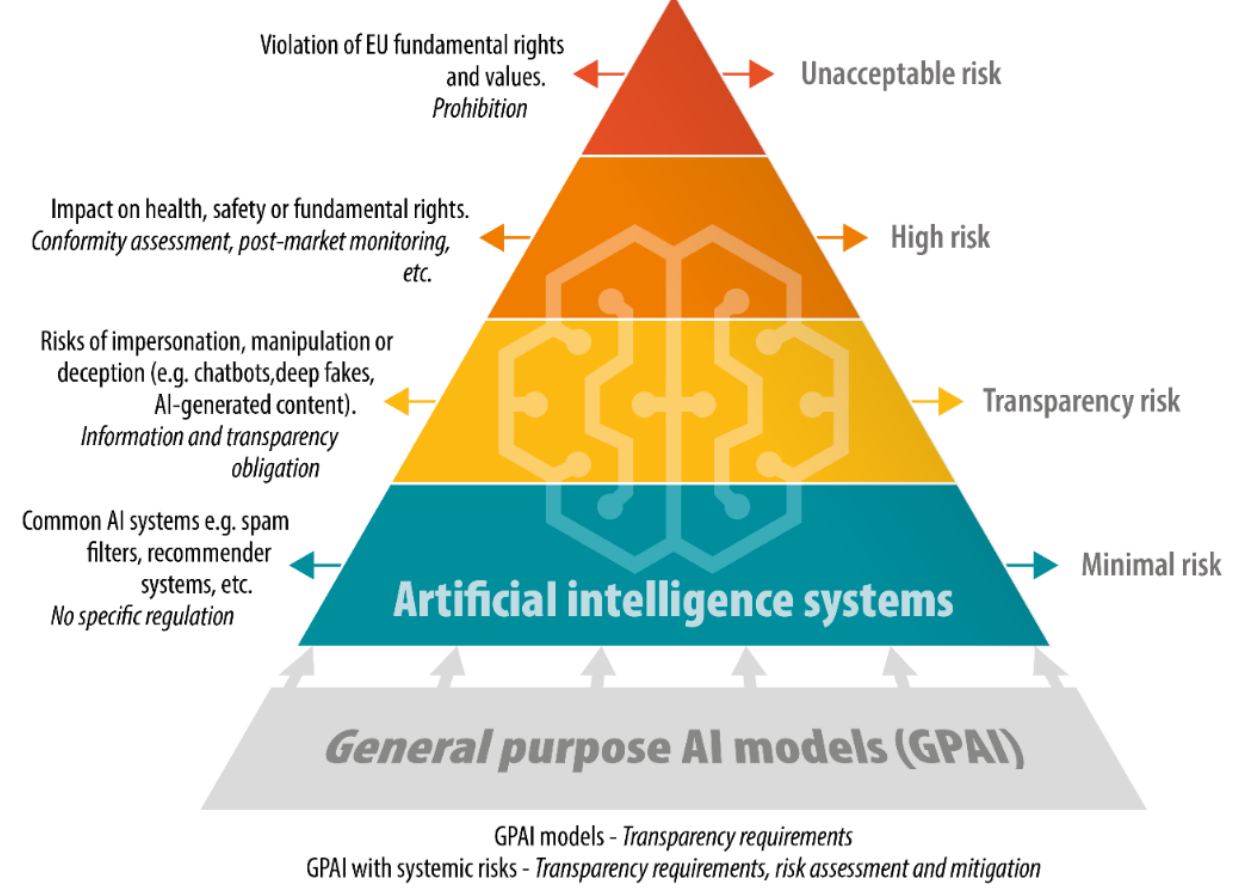
\includegraphics[width=\textwidth]{screen2.png}
\caption{Attaching the tidyverse packages in R}
\label{fig:tidyverse}
\end{figure}

%\section{Tidyverse for Data Analysis}

This section can give only a very brief outline of the capabilities of the tidyverse packages. The extensive documentation and various ''cheat sheets\footnote{\url{https://posit.co/resources/cheatsheets/}} provide additional details. This section focuses on the use of dplyr to analyze data from a set of CSV files representing the data of the Pagila database. The Pagila database\footnote{\url{https://github.com/devrimgunduz/pagila}, \\
\url{https://github.com/devrimgunduz/pagila/blob/master/LICENSE.txt}} is a demonstration database originally developed for teaching and development of the MySQL RDBMS under the name Sakila\footnote{\url{https://dev.mysql.com/doc/sakila/en/}, \\
\url{https://dev.mysql.com/doc/sakila/en/sakila-license.html}}. Pagila is designed as a sample database to illustrate database concepts and is based on a fictional DVD rental store. It originally consists of several tables organized into categories like film and actor information, customer data, store inventory, and rental transactions. For this section, the Pagila data was summarized in a few related CSV files. 

When reading CSV files with readr, the data is stored in a \emph{tibble}\index{Tibble}, not a data frame. A tibble provides a number of extensions and convenience operations that make it significantly more capable than a data frame. When using data frames with dplyr, they are automatically converted to tibbles. 

The following R code reads a CSV file using the \texttt{read\_csv()} function and prints the first few lines and a summary. The output looks slightly different than that for data frames, but accomplishes essentially the same things.

\begin{samepage}
\begin{Rcode}
rentals <- read_csv('rentals.csv')
head(rentals)
summary(rentals)
\end{Rcode}
\end{samepage}

Attaching a tibble or data frame with \texttt{attach()} means that its columns become variables in the R workspace and need not be selected from the tibble (or data frame) using the \texttt{\$} operator. The following R code block transforms the data read from the CSV file into the rentals tibble into appropriate data types, then detaches the tibble and prints a summary.

\begin{samepage}
\begin{Rcode}
# Fix the column datatypes:
attach(rentals)
rating <- as.factor(rating)
language <- as.factor(language)
customer_address <- as.integer(customer_address)
customer_store <- as.integer(customer_store)
rental_staff <- as.integer(rental_staff)
payment_staff <- as.integer(payment_staff)
rental_duration <- as.integer(rental_duration)
detach(rentals)
summary(rentals)
\end{Rcode}
\end{samepage}

The tidyverse libraries make extensive use of the \emph{pipe}\index{Pipe} operator in R. The pipe operator allows chaining of function calls and plugs the result of one function as the first argument into the next function. Originally, tidyverse used the \texttt{\%>\%} pipe operator from the \texttt{magrittr} library, but can now also be used with the new (since R version 4.1), native R pipe operator \texttt{|>}. For simple usage, the two behave identically and can be intermixed. 

The following R code block demonstrates a simple sequence of data manipulation operations using functions from the dplyr library. It begins with the data tibble which is piped into the first function. The outputs of each function are piped into the following function, ending with \texttt{print()}. Note that print output can also be piped into other functions, allowing printing of intermediate results. 

\begin{samepage}
\begin{Rcode}
rentals |> 
  filter(if_any(everything(), is.na)) |>
  select(last_name, rental_date, return_date, title, amount) |>
  print(n=Inf, width=Inf)
\end{Rcode}
\end{samepage}

\begin{itemize}
\item The \texttt{filter(if\_any(everything(), is.na))} function is the first in the pipeline. It filters rows in the rentals data frame based on the presence of NA (missing) values. The \texttt{if\_any()} function checks each column (indicated by \texttt{everything()}) for NA values. The filter function then retains only those rows that have at least one NA value in any column.

\item Next, the \texttt{select()} function specifies the columns to retain in the resulting data frame. It narrows down the data frame to include only the last\_name, rental\_date, return\_date, title, and amount columns. This step reduces the dataset to focus on these key variables, for easier analysis and reporting.

\item Finally, the \texttt{print(n=Inf, width=Inf)} function displays the output. The \texttt{n=Inf} argument tells R to print all rows of the data frame, instead of just the first few rows as is the default behavior. Similarly, \texttt{width=Inf} ensures that all columns are printed without any being truncated, which is useful for wide tibbles or data frames.
\end{itemize}

In summary, this R code example is used to filter a rentals table for rows containing missing values in any column, and then to select and print specific columns of interest. This kind of operation is typical in data cleaning and exploratory data analysis processes. The result shows that some films have not been rented (i.e. there is no rental date for them), and some rentals have not been returned (i.e. there is no return date for them).

The following paragraphs show examples of further data analysis with Tidyverse, introducing additional dplyr functions and their use. Dplyr functions are intended to mirror the SQL queries from the earlier chapter on relational databases. The main dplyr ''verbs'' used in the examples are summarized in Table~\ref{tab:dplyr}. 

\begin{table}
\centering
\renewcommand{\arraystretch}{1.25}

\begin{tabularx}{\textwidth}{l|X} \hline
\texttt{full\_join} & Joins tibbles (also \texttt{outer join}, \texttt{left\_join}, \texttt{inner\_join}, \texttt{right\_join}) \\
\texttt{filter} & filters by row \\
\texttt{select} & selects columns to retain \\
\texttt{mutate} & creates new columns \\
\texttt{rename} & renames columns \\
\texttt{distinct} & finds unique values \\
\texttt{group\_by} & groups data \\
\texttt{nest} & nests data, tibbles in tibbles \\
\texttt{arrange} & sorts data rows \\
\texttt{relocate} & moves data columns \\
\texttt{print} & prints a tibble \\ \hline
\end{tabularx}
\caption{Important dplyr functions}
\label{tab:dplyr}
\end{table}


\paragraph*{Example:} Find all films and the actors that appeared in them, ordered by film category and year, for those films that are rated PG.

\begin{samepage}
\begin{Rcode}
actors <- read_csv('actors.categories.csv')

rentals |> 
  full_join(actors, by='title', 
    suffix=c('_customer', '_actor'), 
    relationship='many-to-many') |>
  filter(rating == 'PG') |>
  mutate(actor = 
    paste(last_name_actor, ', ', first_name_actor, sep='')) |>
  rename(year=release_year) |>
  select(actor, title, category, year) |>
  distinct(actor, title, category, year) |>
  group_by(category, year, title) |> 
  nest() |>
  arrange(category, year, title) |>
  relocate(category, year, title) |>
  print(n=Inf, width=Inf)
\end{Rcode}
\end{samepage}

This R code processes the rentals tibble and the actors tibbles through a sequence of functions in a pipeline.
\begin{itemize}
\item The \texttt{read\_csv()} function is used to read data from a CSV file named ''actors.categories.csv'' into an R data frame called ''actors''.
\item The ''rentals()'' data frame is combined with the ''actors'' data frame using a full join. The join is performed on the ''title'' column common to both data frames. The \texttt{suffix} argument adds distinct suffixes to column names from each data frame to avoid name clashes. The \texttt{relationship='many-to-many'} indicates the nature of the join.
\item The \texttt{filter()} on the combined data retains only rows where the ''rating'' column has the value ''PG''.
\item The \texttt{mutate()} function is used to create a new column named ''actor'', which concatenates the actor's last name and first name, separated by a comma and a space.
\item The ''release\_year' column is renamed to 'year' using the \texttt{rename} function.
\item The \texttt{select()} function is used to narrow down the data frame to only the columns ''actor'', ''title'', ''category'', and ''year''. 
\item Following this, the \texttt{distinct()} function ensures that only unique rows are retained, removing any duplicates.
\item The data is grouped by ''category'', ''year'', and ''title'', and then \texttt{nest} is used to create a nested data frame, i.e. a dataframe where the actors for each group are in a list-valued columns.
\item the \texttt{arrange()} sorts the data frame by ''category'', ''year'', and ''title'', while \texttt{relocate} moves these columns to the front of the data frame for easier viewing.
\item Finally, the entire data frame is printed with all rows (\texttt{n=Inf}) and without truncating any columns (\texttt{width=Inf}).
\end{itemize}


\paragraph*{Example:} Find the most popular actors in the rentals in each city.

This R code block below involves combining multiple data frames and then manipulating and summarizing the data. It builds on the reantal and actor tibbles from the previous example and includes address information.

\begin{samepage}
\begin{Rcode}
addresses <- read_csv('addresses.csv')
addresses$phone <- as.character(addresses$phone)

full_data <- 
  rentals |> 
    inner_join(addresses, by=c('customer_address'='address_id')) |>
    inner_join(actors, by='title',
      suffix=c('_customer', '_actor'),
      relationship='many-to-many')
       
full_data |> 
  mutate(actor = 
    paste(last_name_actor, ', ', first_name_actor, sep='')) |>
  group_by(city, actor) |>
  summarize(count=n()) |>
  mutate(ranking = min_rank(desc(count))) |>
  filter(ranking < 4) |>
  arrange(city, ranking, actor) |>
  print(n=25)
\end{Rcode}
\end{samepage}

\begin{itemize} 
\item The analysis starts by reading a CSV file containing addresses into a data frame.
\item An inner join is first performed between these two data frames, matching them on a specified key. 
\item This is followed by another inner join with an `actors` data frame. This second join involves a many-to-many relationship and adds suffixes to overlapping column names to distinguish them.
\item With the full data set, a new column is created by concatenating the first and last names of actors, forming complete names. 
\item The data is then grouped by city and actor.
\item A new summary column is created that counts the number of occurrences (records) for each group.
\item To create rankings, a new column is added that ranks the groups based on the count in descending order. The \texttt{min\_rank()} function allows ties in the ranking, use \texttt{rank()} to break ties with gaps in ranking or \texttt{dense\_rank()} to break ties with no gaps in ranking.
\item The data is then filtered to include only those records with a ranking less than 4, focusing on the top three ranks for each group.
\item Finally, the data is sorted by city, ranking, and actor and then printed.
\end{itemize}


\paragraph*{Example:} Find the customers who spend the most on rentals, with their phone numbers and cities, and the number of rentals with the higest total rental payments for each category grouped by rental duration.

\begin{samepage}
\begin{Rcode}
full_data |>
   mutate(customer= paste(first_name_customer, last_name_customer)) |>
   select(customer, amount, rental_duration, category, phone, city) |>
   group_by(category, rental_duration, customer ) |>
   mutate(payments=sum(amount), num_rentals=n()) |>
   select(-amount) |>
   group_by(category, rental_duration) |>
   mutate(ranking = min_rank(desc(payments))) |>
   slice(which.min(ranking)) |>
   print(n=Inf, width=Inf)
\end{Rcode}
\end{samepage}

By now, it should be clear what the functions in the analysis pipelines accomplish. However, a few interesting things to note. First, there is no \texttt{summarize()} function because \texttt{summarize()} omits all non-grouped columns, but the example requires phone numbers and citites of customers. Either these would need to be included somehow in the \texttt{summarize()} function, or as is done in this R code, summary columns are created with \texttt{mutate()}. Second, note the ''negative'' argument to the \texttt{select()} function, which is used to remove the ''amount'' column. Third, the pipeline uses multiple \texttt{group\_by()} statements with different aggregate functions (\texttt{sum()}, \texttt{n()}, \texttt{min\_rank()}) for the different groups. Finally, the R code uses \texttt{slice()} to select the rows with the smallest ranks.

\paragraph*{Example:} Get the total rental revenue, number of rentals, and the mean and standard deviation of the rental amounts for each country.

\begin{samepage}
\begin{Rcode}
full_data |>
  group_by(country) |>
  summarize(revenue=sum(amount), 
            numrentals=n(),
            mean_amount=mean(amount),
            sd_amount=sd(amount)) |>
  arrange(desc(mean_amount),
          desc(revenue)) |>
  print(n=Inf, width=Inf)  
\end{Rcode}
\end{samepage}

The R code for this query demonstrates a number different aggregate summary functions, \texttt{sum()}, \texttt{n()}, \texttt{mean()} and \texttt{sd()} (standard deviation). It also shows how to use the \texttt{desc()} function to arrange or sort data in decreasing order.

\paragraph*{Example:} Get the top 5 and the bottom 5 grossing customers for each quarter.

\begin{samepage}
\begin{Rcode}
full_data |>
  mutate(customer=paste(first_name_customer,last_name_customer)) |>
  mutate(q=as.character(quarter(rental_date, with_year=T))) |>
  select(customer, q, amount, rental_date) |>
  group_by(q, customer) |>
  mutate(payments=sum(amount)) |>
  select(-amount) |>
  distinct(customer, q, payments) |>
  group_by(q) |>
  mutate(rank_top = min_rank(desc(payments))) |>
  mutate(rank_bot = min_rank(payments)) |>
  filter(rank_top < 6 | rank_bot < 6) |>
  arrange(q, desc(payments)) |>
  relocate(q, customer, payments, rank_top, rank_bot) |>
  print(n=Inf, width=Inf)
\end{Rcode}
\end{samepage}

The code for this query again does not use a \texttt{summarize()} function. It also shows the use of the \texttt{quarter()} function from the ''lubridate'' library. The lubridate library contains a large range of date and time related functions. Two ranking columns are created using the \texttt{mutate()} and \texttt{min\_rank()} functions, once in descending order to get the top ranks, and again in ascending order to get the bottom ronks. The code uses \texttt{filter()} instead of \texttt{slice()} to select the top and bottom 5 ranks, uses \texttt{arrange()} to sort the data, and then uses \texttt{relocate()} to re-arrange the order of columns prior to printing.

\paragraph*{Example:} Find the set of film titles by rental customer and the total number rentals for each customer.

\begin{samepage}
\begin{Rcode}
full_data |>
  mutate(customer=paste(first_name_customer,last_name_customer)) |>
  select(customer, title) |>
  nest(titles=title) |>
  rowwise() |> 
  mutate(rentals=nrow(titles)) |>
  mutate(unique_titles=list(distinct(titles))) |>
  select(-titles) |>
  arrange(customer) |>
  print(n=Inf, width=Inf)
\end{Rcode}
\end{samepage}

The code for this query works with nested data, that is, data with columns that contain lists, created using the \texttt{nest()} function. In this example, \texttt{nest(titles=title)} creates a columns called ''titles'' that contains a list of all the elements of the ''title'' column for each customer. The R code also demonstrates row-wise operations. Both \texttt{mutate()} functions after \texttt{rowwise()} function operate by row. Specifically, the first use of the \texttt{mutate()} function creates a new column ''rentals'' which contains the number of rows in the titles column \emph{for each row} (recall that the ''titles'' column contains lists of film title). Similarly, the second use of the \texttt{mutate()} function creates a new column ''unique\_title''that contains a list of distinct film titles from the ''titles'' column \emph{for each row}.

\section{SQL and R}

The ''sqldf'' library in R allows users to perform SQL queries on R data frames. Essentially, it provides a bridge between SQL and R\index{SQL!in R}. This integration allows users who are familiar with SQL to leverage its powerful querying capabilities directly on R data structures, without the need to switch between different tools or environments.

One of the main advantages of ''sqldf'' is its ability to handle large data frames more efficiently than some of R's native functions. By utilizing SQL queries, users can perform complex data manipulations and aggregations with ease. The package supports various SQL commands including SELECT, JOIN, ORDER BY, and GROUP BY, among others, enabling a wide range of data operations that are familiar to SQL users.

Under the hood, ''sqldf'' operates by temporarily converting data frames into databases, typically by creating an in-memory SQLite database, or, alternatively, using an existing database connection to any of a variety of RDBMS such as PostgreSQL. It then creates a table for each data frame, moves the data to the database tables, and executes SQL statements. It then moves the result set back into R as a data frame. This seamless process allows for a smooth integration of SQL's data processing capabilities within the R environment.

''sqldf'' is particularly useful for R users who are already comfortable with SQL syntax and for complex data manipulation tasks that might be more cumbersome or less intuitive in R's native syntax. Its ability to handle data frames as if they were SQL tables makes it a highly valuable tool for data analysts and statisticians who work with large datasets and require the flexibility and power of SQL within the R programming environment.

The following R code block shows a very simple example. Note that the SQL \texttt{FROM} clause recognizes data frame names; any columns used in the SQL query must be named columns from those data frames.

\begin{Rcode}
library(sqldf)
result_df <- sqldf('select distinct(title) from full_data')
\end{Rcode}

When faced between the choice of data analytics using an SQL RDBMS or R/Tidyverse, there are a number of issues to consider:

\begin{itemize}
 \item \emph{Size of data}: R is limited by the amount of main memory of the computer. While large computers may offer 128GB or more, modern RDBMS can scale massively larger, in particular when distributing databases across a cluster of computers.
 \item \emph{Access speed}: RDBMS have sophisticated indexing of tables and query planners that optimize complex queries for performance. While a dplyr analysis pipeline can also be optimized by carefully considering the order of function calls, the onus is on the data analyst to do this, while an RDBMS offer this ''out-of-the-box''.
 \item \emph{Currency}: Using an RDBMS means that analytics can be performed on operational data, that is, the most current and up-to-date data. In contrast, the use of R involves first exporting data from the operational system and then analyzing it at a later time. However, while tempting, it is not generally recommended to perform complex analytics on an operational database, as it can significantly affect performance. 
 \item \emph{Transactions}: An RDBMS ensures consistent views of data across multi-user, concurrent updates. This means that, when using an operational database, the analysis sees consistent data, whereas an exported snapshot of the data may not necessarily be consistent, depending on the export mechanism.
 \item \emph{Tools}: R has tools for statistical analysis and visualization, beyond mere reporting. So far, we have considered only simple descriptive analytics. However, when the data is to be used for sophisticated statistics or predictive analytics, it is no longer possible to do this on RDBMS.
\end{itemize}

\noindent These issues motivate the following recommendations:
\begin{itemize}
 \item Do not ''hit'' operational RDBMS for heavy-weight or frequent analytics. While it may be fine to do the occasional summary analytics on an operational database, this should not be normally done. 
 \item Regularly export consistent data from RDBMS. If up-to-date data is needed, automate the export from the database to occur at regular intervals. However, note also that exporting data has a performance impact on operational databases. 
 \item Sometimes, SQL may be the more intuitive language to specify the required analysis. In these cases, use separate in-memory or on-disk RDBMS for analytics (e.g. with \texttt{sqldf}) if desired/required. 
 \item Finally, if the size of data is too large to handle in R, consider distributed tools such as Hadoop/Spark that are made for Big Data analytics.
\end{itemize}

\begin{tcolorbox}[colback=code]
\subsection*{Hands-On Exercises}

The following hands-on exercises are designed to familiarize you with the Tidyverse packages, especially the dplyr package. Use these exercises with the Pagila CSV data set.

\begin{enumerate}[nosep]
  \item Find all films with a rating of 'PG'
  \item List all customers who live in Canada (with their address)
  \item Find the average \emph{actual} rental duration for all films
  \begin{itemize}
     \item This requires date arithmetic, use the \texttt{lubridate} package
  \end{itemize}
  \item Find the average overdue time for each customer
  \begin{itemize}
     \item This requires date arithmetic, use the \texttt{lubridate} package
  \end{itemize}
  \item List all films that have never been rented
  \item List the names of actors who have played in more than 15 films
\end{enumerate}
\end{tcolorbox}
